\setcounter{chapter}{-1}

\begin{chapter}{Introduction}
 Structure:
 \begin{enumerate}
     \item goal of the report
     \item What is machine learning
     \item supervised machine learning
     \item kernel methods
     \item main results in kernel methods theory
 \end{enumerate}
 The goal of the present work is to further investigate the capabilities of kernel methods in the context of memory-constrained systems.
 We will explore the theoretical foundations of kernel methods, adapting previous work done in the Random Fourier Features framework, analyze their performance in various scenarios,
 and propose novel approaches to optimize their efficiency while maintaining high accuracy. In particular we
 will focus on the quantization of kernel methods, which is a promising avenue for reducing memory usage without significantly compromising performance.
 We apply this technique in an empirical loss minimization setting, exploiting mini-batches SGD algorithms, and we show that it can achieve competitive results compared to unquantized methods,
 while significantly reducing memory requirements.
 We start with a brief introduction to machine learning, supervised learning, and kernel methods, before delving into the main results of our work.

 \begin{figure}
     \centering
     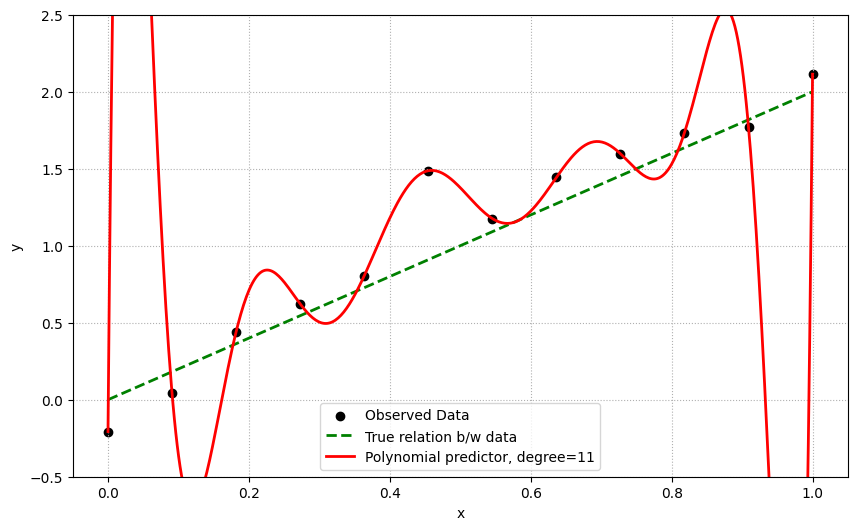
\includegraphics[width=0.8\textwidth]{pics/0-data_overfitting.png}
     \caption{Example of overfitting: the model fits the training data perfectly but fails to generalize to new data, which are distrubuted as: $ y = 2x + \epsilon$, where $\epsilon$ is a Normal noise term.}
     \label{0-data_overfitting}
 \end{figure}
 \begin{section}[Machine Learning]{Overview of Machine Learning }
  Machine learning is a subfield of artificial intelligence that focuses on the development of algorithms and statistical models that enable
  computers to perform tasks without previous coded instructions. The core idea behind machine learning is to allow systems to learn from data, identify patterns, and make decisions with minimal human intervention on
  data not previously seen. Machine learning algorithms can be broadly categorized into three main types: supervised learning, unsupervised learning, and reinforcement learning.
  We are going to focus on supervised learning, which is the most widely used type of machine learning, where the algorithm is trained on a labeled dataset, meaning that each training example is paired with an output label.
  \vspace{5pt}
  \newline Assume we have a dataset of $n$ examples, where each example consists of an input vector $x_i \in \mathbb{R}^d$ and a corresponding output label $y_i \in \mathbb{R}$.
  The goal of supervised learning is to learn a function $f: \mathbb{R}^d \rightarrow \mathbb{R}$ that can predict the output label $y$ for new, unseen input vectors $x$.
  To do so, we "train" the model by minimizing a loss function that measures the discrepancy between the predicted outputs and the true labels in the training data, i.e. we solve the following optimization problem:
  \begin{equation}
      \min_{f \in \mathcal{H}} \frac{1}{n} \sum_{i=1}^n L(f(x_i), y_i) + \lambda R(f)
  \end{equation}
  where $\mathcal{H}$ is a suitable space of functions (predictors), $L$ is a loss function that quantifies the error of the predictions, $R$ is a regularization term, i.e. it prevents $f$ from varing too sharply in order to fit
  the knonwn data hence only "memorizing" it, and $\lambda$ is a regularization parameter that controls the trade-off between fitting the training data and keeping the model simple.
  One of the most common choiches for the function $L$ is the mean squared error, defined as $L(f(x_i), y_i) = (f(x_i) - y_i)^2$, which is widely used for regression problems and the one
  we will be using in this work. A common choiche for the regularization term $R$ is the squared norm of $f$ in a suitable function space, which is known as Tikhonov regularization and is widely used in kernel methods.
  \vspace{5pt}
  \newline As previously mentioned, choosing the right function space $\mathcal{H}$ is crucial for the success of the learning algorithm.
  If the space is too large, in a sense that we will further clarify in the next sections, the model may overfit the training data, meaning that it will perform well on the training data but poorly on new, unseen data.
  On the other hand, if the space is too small, the model may underfit the training data, meaning that it will perform poorly on both the training data and new, unseen data.
  It is also important to work with a function space that allows for efficient optimization, as the training process involves solving an optimization problem, which could be unfeasible if the function space is too complex.
  In the example given in Figure \ref{0-data_overfitting} we allow the function space to include higly interpolating polynomials, which leads
  to a zero training error but once evaluated on new data, the model fails to generalize and performs poorly, which is a clear example of overfitting.
  \vspace{5pt}
  \newline We give now more formal definitions.
  \begin{definition}
      Let $\mathcal{X} \subseteq \R^d $ be the input space and $\mathcal{Y} \subseteq \R$ the output space. Over the
      product space $\mathcal{X} \times \mathcal{Y}$ we assume there is a probability distribution function $\rho$ that generates the data, and we denote by $\rho_x$ the marginal distribution of $\rho$ on $\mathcal{X}$
      and with $\rho(y|x)$ the conditional distribution of $\rho$ given $\mathcal{X}$.
  \end{definition}
  As previously mentioned, the goal of supervised learning is to learn a function \newline $f: \mathcal{X} \rightarrow \mathcal{Y}$ that can predict the output label $y$ for new, unseen input vectors $x$;
  so the next definition comes naturally:
  \begin{definition}
      Let $\mathcal{H}$ a space of function from $\mathcal{X}$ to $\mathcal{Y}$, each of the function $f$ in $\mathcal{H}$ is called a predictor.
  \end{definition}
  Now we define the quantity with respect to which we choose the best predictor:
  \begin{definition}
      A function $l : \mathcal{Y} \times \mathcal{Y} \to \R_{\geq 0}$ is called loss function. The most common loss function is
      the mean squared error, defined as:
      $$
          l(y', y) \coloneqq ||y'-y||^2
      $$
  \end{definition}
  \begin{definition}
      We call expected risk the function:
      $$
          R(f) \coloneqq \E_\rho(l(f(x), y)) = \int_{\mathcal{X}\times \mathcal{Y}}l(f(x), y) d\rho(x,y)
      $$
      where $f \in \mathcal{H}$ suitable function space.
  \end{definition}
  The best predictor in $\mathcal{H}$ is defined as the minimizer of the expected risk function.
  Theoretically the best possible predictor is the following:
  \begin{definition}
      We call Bayes Predictor the function:
      $$f^\star(x) = \argmin_{z \in \mathcal{Y}}\E_{y \sim \rho(y|x)}(l(y, z))$$
      and the corresponding risk is called Bayesian Risk, which is the best theoreticaly achievable risk\footnote{This can be easily seen, since $d\rho_X$ is a positive measure.}:
      $$
          R(f^\star) = \E_{x \sim \rho_X}\left(\inf_z \E_{y \sim \rho(y|x)} (l(z, y))\right)
      $$
  \end{definition}
  It is clear that we do not have access to $\rho$, otherwise we could (numericaly) compute the function $f^\star$ and get a state-of-the-art predictor. Since we do not have $\rho$, we cannot even
  calculate $R(\cdot)$; we have then to rely on the following:
  \begin{definition}
      Let $(x_i, y_i)_{i=1, \dots, n} \in \mathcal{X}\times \mathcal{Y}$ be the known dataset, let $f$ an estimator. We define
      the Empirical Risk as:
      $$
          \hat{R}(f) = \frac{1}{n}\sum_{i=1}^n l(f(x_i), y)
      $$
  \end{definition}
  The minimization of the empirical risk is a core idea behind the majority of machine learning tasks.
  \vspace{5pt}
  \newline When learning the best regressor, with respect to the choosen loss, an ideal situation would be it to be a linear
  function, hence easier to learn in computational framework. Unfortunatly this is not always the case, but there are
  tecniques to non-linear regression that allow us to tackle this issue. The main idea is to map the input space to a higher
  dimensional space where the data is more likely to be linearly separable, and then learn a linear regressor in this higher dimensional space.
  The problem of choosing the right function space is know as model selection, and it is a crucial aspect of supervised learning.




 \end{section}

 \begin{section}{Kernel Methods}
  We star defining a kernel function:
  \begin{definition}
      Let $\mathcal{X} \subseteq \R^d$ be the input space, we call kernel function, a simmetric function $k: \mathcal{X}\times \mathcal{X} \to \R$ s.t. for all $n \in \mathbb{N}, x_1, \dots, x_n \in \mathcal{X}$ and $c_1, \dots, c_n \in \R$, we have:
      $$
          \sum_{i=1}^n \sum_{j=1}^n c_i c_j k(x_i, x_j) \ge 0
      $$
  \end{definition}
  This last condition is called positive semi-definiteness and it ensures that the matrix of the kernel values, called Gram matrix, is positive semi-definite. It is related to the definition of
  a kernel function through the following theorem:
  \begin{theorem}
      Let $\mathcal{X} \subseteq \R^d$ be the input space and $k: \mathcal{X}\times \mathcal{X} \to \R$ a simmetric function. Then $k$ is a kernel function if and only if there exists a Hilbert space $\mathcal{H}$ and a feature map $\phi: \mathcal{X} \to \mathcal{H}$ such that for all $x, y \in \mathcal{X}$:
      $$
          k(x, y) = \langle \phi(x), \phi(y) \rangle_{\mathcal{H}}
      $$
      where $\langle \cdot, \cdot \rangle_{\mathcal{H}}$ denotes the inner product in $\mathcal{H}$. In this
      case $\mathcal{H}$ is called Reproducing Kernel Hilbert Space, and the map $\phi$ is
      called feature map.
  \end{theorem}
  The theorem, due to Aronszajn in the 1950s, allows us to implicitly map the data to a higher
  dimensional space where it is more likely to be linearly separable, furthermore, as we are about to see, we do not
  need to know the explicit feature map, since most of the algorithms rely only on the "interaction between data", i.e. the value
  of the kernel function.
  \vspace{5pt}
  \newline To see the link with learning theory we need some assumption. First we assume our predictors to be
  linear with respect to the parameters, i.e. of the form:
  $$
      f_\theta: \mathcal{X}\rightarrow \R, \quad x \to \langle \theta, \phi(x) \rangle_{\mathcal{H}}
  $$
  where $\theta \in \mathcal{H}$ is the parameter vector. Note that the function is not linear on the data $x$ itself, but
  on their representation in the feature space $\mathcal{H}$. Furthermore we assume the loss function to be of the form: 
  $$
    L(f_\theta, (x_i, y_i)_{i=1,\dots,n}) = \frac{1}{n}\sum_{i=1}^n l(f_\theta(x_i), y_i) + \lambda ||\theta||^2
  $$
  where $l$ is a loss function and $\lambda \geq 0$ is the regularization parameter. 
  Now we can state the following theorem, which allows us to restrict the optimal parameters space.

  \begin{theorem}
      Consider a feature map $\phi : \mathcal{X} \rightarrow \mathcal{H}$. Let
      $(x_1,\dots,x_n) \in \mathcal{X}^n$, and assume that the functional $\Psi : \R^{n+1} \rightarrow \R$ is strictly increasing
      with respect to the last variable. Then the infimum of
      $$
          \Psi\left(\theta, \phi(x_1), \dots, \phi(x_n), ||\theta||^2\right)
      $$
      can be obtained by restricting to a vector $\theta$ in the span of $\phi(x_1), \dots, \phi(x_n)$ ; that is, of the
      form
      $$
          \theta = \sum_{i=1}^n \alpha_i \phi(x_i)
      $$
      with $\alpha \in \R^n$.
  \end{theorem}
  It comes straightforward that the loss function we defined above satisfies the hypothesis of the theorem, hence 
  we can restrict our search space of optimal parameters to the space spanned by the feature map of the training data.
  \vspace{5pt}
  \newline 
  \begin{subsection}{Translation Invariant Kernels}
    We now focus on a translation invariant kernels, which will be the starting point of this work.
  \end{subsection}
 \end{section}



\end{chapter}